\section{Thiết kế và thực hiện}

\subsection{Thiết kế node BLE từ chip EPS32-C3}

\subsubsection{Sensor}

Nhóm sử dụng \textbf{DHT11 Humidity \& Temperature Sensor} cho Node. Với DHT11 Sensor có chức năng vừa đo độ ẩm và nhiệt độ. Thực hiện bằng giao thức one-wire serial interface.

\begin{figure}[H]
	\centering
	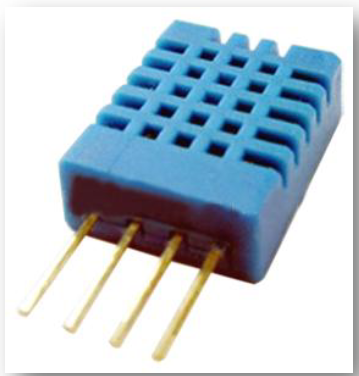
\includegraphics[width=.3\linewidth]{./my-chapters/my-images/implementation/Node/DHT11_picture.png}
	\caption{Hình ảnh cảu DHT11.}
\end{figure}

Với thiết kế nhỏ gọn, tiêu thụ công suất thấp và có thể truyền tín hiệu lên tới 20m. 

\noindent\textbf{Overview}
		\begin{table}[H]
				\centering
				\begin{tabular}{|>{\centering\arraybackslash}m{1.5cm}
								|>{\raggedright\arraybackslash}m{2.5cm}
								|>{\raggedright\arraybackslash}m{2.5cm}
								|>{\raggedright\arraybackslash}m{2.5cm}
								|>{\raggedright\arraybackslash}m{2.5cm}
								|>{\raggedright\arraybackslash}m{2.5cm}|}
							\hline
						Item & Measurement Range & Humiidity Accuracy & Temperature Accuracy & Resolation & Package \\ \hline 
						DHT11 & $20-90 \%$ RH $0-50^{o}C$ & $\pm 5\%$ RH & $\pm 2^{o}C$ & 1 & 4 Pin Single Row \\ \hline
					\end{tabular}
			\end{table}
%\noindent\textbf{Technical Specifications}
%
%\begin{itemize}[label=-]
%	\item Overview:
%		\begin{table}[H]
%			\centering
%			\begin{tabular}{|>{\centering\arraybackslash}m{1.5cm}
%					|>{\raggedright\arraybackslash}m{2.5cm}
%					|>{\raggedright\arraybackslash}m{2.5cm}
%					|>{\raggedright\arraybackslash}m{2.5cm}
%					|>{\raggedright\arraybackslash}m{2.5cm}
%					|>{\raggedright\arraybackslash}m{2.5cm}|}
%					\hline
%				Item & Measurement Range & Humiidity Accuracy & Temperature Accuracy & Resolation & Package \\ \hline 
%				DHT11 & $20-90 \%$ RH $0-50^{o}C$ & $\pm 5\%$ RH & $\pm 2^{o}C$ & 1 & 4 Pin Single Row \\ \hline
%			\end{tabular}
%		\end{table}
%	\item Detailed Specifications:
%		\begin{longtable}{|>{\centering\arraybackslash}m{3.5cm}
%				|>{\centering\arraybackslash}m{4cm}
%				|>{\centering\arraybackslash}m{3cm}
%				|>{\centering\arraybackslash}m{3cm}
%				|>{\centering\arraybackslash}m{3cm}|}
%			\caption{Typical Humidity and Temperature Characteristics} \label{tab:ht_specs} \\
%			\hline
%			\textbf{Parameters} & \textbf{Conditions} & \textbf{Minimum} & \textbf{Typical} & \textbf{Maximum} \\ \hline
%			\endfirsthead
%			
%			\multicolumn{5}{c}%
%			{{\tablename\ \thetable{} -- continued from previous page}} \\
%			\hline
%			\textbf{Parameters} & \textbf{Conditions} & \textbf{Minimum} & \textbf{Typical} & \textbf{Maximum} \\ \hline
%			\endhead
%			
%			\hline \multicolumn{5}{r}{{Continued on next page}} \\
%			\endfoot
%			
%			\hline
%			\endlastfoot
%			
%			\multicolumn{5}{|c|}{\textbf{Humidity Characteristics}} \\ \hline
%			Resolution & -- & 1\%RH (8 Bit) & 1\%RH (8 Bit) & 1\%RH (8 Bit) \\ \hline
%			Repeatability & -- & -- & $\pm 1\%$RH & -- \\ \hline
%			Accuracy & 25$^{\circ}$C & -- & $\pm 4\%$RH & -- \\ \hline
%			Accuracy & 0--50$^{\circ}$C & -- & $\pm 5\%$RH & -- \\ \hline
%			Interchangeability & \multicolumn{4}{c|}{Fully Interchangeable} \\ \hline
%			Measurement Range & 0$^{\circ}$C & 30\%RH & -- & 90\%RH \\ \hline
%			Measurement Range & 25$^{\circ}$C & 20\%RH & -- & 90\%RH \\ \hline
%			Measurement Range & 50$^{\circ}$C & 20\%RH & -- & 80\%RH \\ \hline
%			Response Time & 1/e (63\%), 25$^{\circ}$C, 1 m/s Air & 6 s & 10 s & 15 s \\ \hline
%			Hysteresis & -- & -- & $\pm 1\%$RH & -- \\ \hline
%			Long-Term Stability & Typical & -- & $\pm 1\%$RH/year & -- \\ \hline
%			
%			\multicolumn{5}{|c|}{\textbf{Temperature Characteristics}} \\ \hline
%			Resolution & -- & 1$^{\circ}$C (8 Bit) & 1$^{\circ}$C (8 Bit) & 1$^{\circ}$C (8 Bit) \\ \hline
%			Repeatability & -- & -- & $\pm 1^{\circ}$C & -- \\ \hline
%			Accuracy & -- & -- & $\pm 1^{\circ}$C & $\pm 2^{\circ}$C \\ \hline
%			Measurement Range & -- & 0$^{\circ}$C & -- & 50$^{\circ}$C \\ \hline
%			Response Time & 1/e (63\%) & 6 s & -- & 30 s \\ \hline
%		\end{longtable}
%\end{itemize}

\noindent\textbf{Typical Application}

\begin{figure}[H]
	\centering
	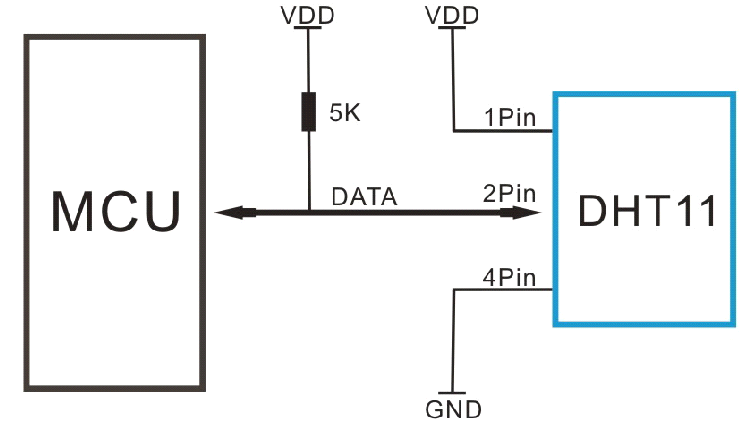
\includegraphics[width=.6\linewidth]{./my-chapters/my-images/implementation/Node/DHT11_connect.png}
	\caption{Typical Application.}
\end{figure}

\noindent\textbf{Power supply}

Điện áp cấp cho DHT11 thông thường dao động từ $3-5.5$ VDC.

\noindent\textbf{Communication Process: Serial Interface (Single-Wire Two-Way)}

Định dạng dữ liệu một đường truyền được sử dụng để giao tiếp và đồng bộ giữa MCU và cảm biến DHT11. Một quá trình giao tiếp mất khoảng $4ms$.

\begin{itemize}[label=-]
	\item Overall Communication Process: Khi MCU gửi tín hiệu hoạt động, DHT11 chuyển từ chế độ tiết kiệm năng lượng sang chế độ hoạt động và chờ MCU hoàn thành tín hiệu bắt đầu. Khi MCU đã hoàn thành thì DHT11 sẽ gửi một tín hiệu xác nhận với 40-bit dữ liệu bao gồm các dữ liệu liên quan đến độ ẩm và nhiệt độ cho MCU.
		\begin{figure}[H]
			\centering
			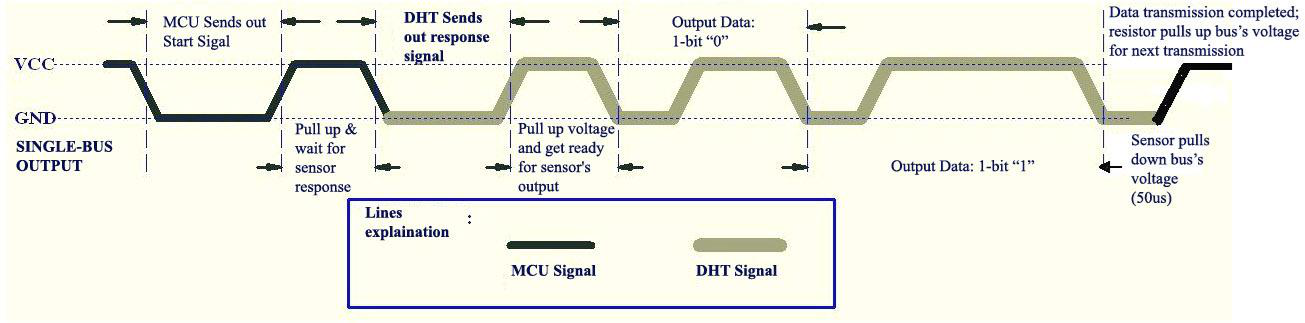
\includegraphics[width=.8\linewidth]{./my-chapters/my-images/implementation/Node/overall_communication_process.png}
		\end{figure}
	\item MCU Sends out Start Signal to DHT: Nếu không hoạt động thì đường dây Data sẽ luôn ở mức cao. Nếu có tín hiệu cần giao tiếp giữa MCU và DHT11 thì MCU sẽ kéo điện áp trên đường dây Data từ 1 xuống 0 trong khoảng ít nhất $18ms$ để đảm bảo DHT nhận được tín hiệu start từ MCU, sau đó MCU sẽ kéo lên 1 trong khoảng $20-40us$.
		\begin{figure}[H]
			\centering
			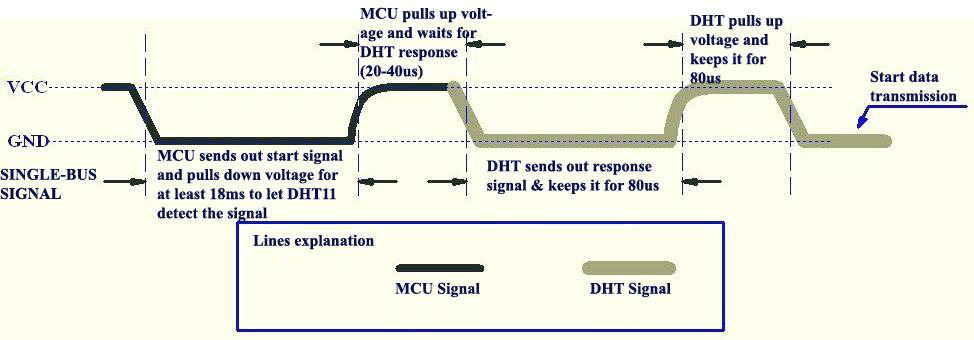
\includegraphics[width=.6\linewidth]{./my-chapters/my-images/implementation/Node/mcu_send_data.png}
		\end{figure}
	\item DHT Responses to MCU: Khi DHT nhận được tín hiệu start, nó sẽ gửi lại một tín hiệu xác nhận low-voltage-level với khoảng $18ms$. Sau đó, chương trình của DHT đặt mức điện áp của đường dữ liệu đơn từ thấp lên cao và giữ trong $80us$ để DHT chuẩn bị gửi dữ liệu.
		\begin{figure}[H]
			\centering
			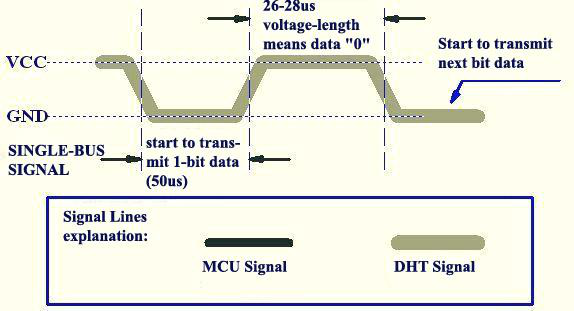
\includegraphics[width=.4\linewidth]{./my-chapters/my-images/implementation/Node/data_0_indications.png}
			\caption{Data "0" indication.}
		\end{figure}
		\begin{figure}[H]
			\centering
			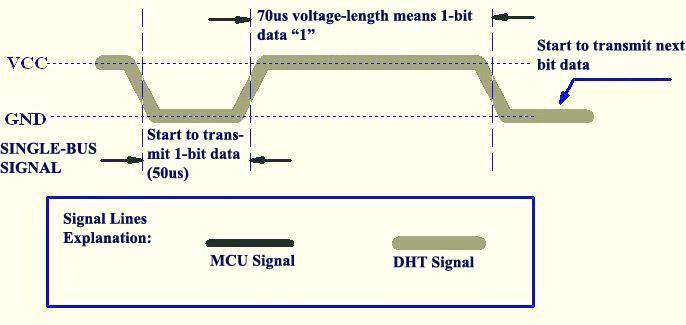
\includegraphics[width=.4\linewidth]{./my-chapters/my-images/implementation/Node/data_1_indications.png}
			\caption{Data "1" indication.}
		\end{figure}
\end{itemize}

\noindent\textbf{Thực thi đọc dữ liệu từ DHT11}

\begin{lstlisting}[style=StyleCode, language=C, caption={Thực thi đọc dữ liệu từ sensor DHT11.}]
	#include <DHT.h>
	
	// ------------------- DHT11 Configuration -------------------
	#define DHTPIN 10
	#define DHTTYPE DHT11
	DHT dht(DHTPIN, DHTTYPE);
	
	void setup() {
		Serial.begin(115200);
		dht.begin();
		
		// --- Read DHT11 sensor data ---
		float temperature = dht.readTemperature();
		float humidity = dht.readHumidity();
	}
\end{lstlisting}

\subsubsection{BLE}

\noindent\textbf{Tổng quan của chương trình}

%\lstinputlisting[style=StyleCode, language=C, caption={Code thực thi chính của BLE sensor node.}]{./my-chapters/my-refs/Code/code.c}

\begin{itemize}[label=-]
	\item \textbf{Advertising BLE:}
	Là quá trình mà ESP32 phát các gói tin quảng bá định kỳ chứa thông tin cơ bản của thiết bị, chẳng hạn như tên thiết bị và UUID của dịch vụ BLE.
	Nhờ vào cơ chế này, các thiết bị xung quanh (ví dụ: smartphone hay laptop) có thể phát hiện và khởi tạo kết nối với ESP32.
	\begin{lstlisting}[style=StyleCode, language=C]
		pServer->getAdvertising()->start();
	\end{lstlisting}
	
	\item \textbf{Notification BLE:}  
	Là quá trình mà thiết bị đóng vai trò Server (ESP32) chủ động gửi dữ liệu cập nhật đến thiết bị Client (ví dụ: điện thoại) mà không cần Client phải gửi yêu cầu đọc.  
	Cơ chế này rất hữu ích để truyền liên tục các giá trị cảm biến theo thời gian thực như nhiệt độ và độ ẩm.  
	\begin{lstlisting}[style=StyleCode, language=C]
		pCharacteristicTX->notify();
	\end{lstlisting}
	
	\item \textbf{Payload BLE:}  
	Là phần dữ liệu thực tế được chứa trong gói tin BLE.  
	Trong hệ thống này, payload bao gồm chuỗi dữ liệu định dạng sẵn, chứa thông tin về nhiệt độ và độ ẩm đo được từ cảm biến DHT11.  
	\begin{lstlisting}[style=StyleCode, language=C]
		pCharacteristicTX->setValue(sensorData);
	\end{lstlisting}
	
\end{itemize}

\noindent\textbf{Quản lý power state (sleep, wake-up, duty cycle)}

\begin{itemize}[label=-]
	\item \textbf{Sleep Mode:} Giảm tiêu thụ năng lượng	thông qua.
	\begin{lstlisting}[style=StyleCode, language=C]
		esp_deep_sleep_start()
	\end{lstlisting}
	\item \textbf{Wake-up Timer:} Tự thức dậy sau một khoảng thời gian.
	\begin{lstlisting}[style=StyleCode, language=C]
		esp_sleep_enable_timer_wakeup()
	\end{lstlisting}
	\item \textbf{Duty Cycle Control:} Giới hạn thời gian hoạt động.
	\begin{lstlisting}[style=StyleCode, language=C]
		void loop() {
			// Not used. After deep sleep, ESP32 restarts and runs setup() again.
		}
	\end{lstlisting}
%	\item \textbf{}
%	\begin{lstlisting}[style=StyleCode, language=C]
%		esp_sleep_enable_timer_wakeup()
%	\end{lstlisting}
\end{itemize}

\noindent\textbf{Ngắt (interrupt) từ GPIO\_WU}

\begin{itemize}[label=-]
	\item \textbf{Setup GPIO:} GPIO\_03 là chân nhận tính hiệu đánh thức từ bộ WuRx (Wake-up Receiver).
	\begin{lstlisting}[style=StyleCode, language=C]
		#define WURX_PIN    3      // External wake-up interrupt from WuRx
	\end{lstlisting}
	\item \textbf{Nguyên nhân đánh thức:} Nếu ESP32-C3 được đánh thức bởi tín hiệu ngắt ngoài (EXT0), thì nguyên nhân là do WuRx kích hoạt thông qua GPIO3. Nếu không, thì là khởi động bình thường (sau reset hoặc cấp nguồn).
	\begin{lstlisting}[style=StyleCode, language=C]
		// --- Check wake-up reason ---
		esp_sleep_wakeup_cause_t wakeup_reason = esp_sleep_get_wakeup_cause();
		if (wakeup_reason == ESP_SLEEP_WAKEUP_EXT0) {
			Serial.println("[SYSTEM] Wake-up triggered by WuRx (GPIO3)");
		} else {
			Serial.println("[SYSTEM] Normal power-up");
		}
	\end{lstlisting}
	\item \textbf{Kích hoạt cơ chế đánh thức:} đánh thức bằng mức tín hiệu thấp (LOW) trên GPIO\_03.
	\begin{lstlisting}[style=StyleCode, language=C]
		// Enable wake-up on GPIO3 (LOW level = wake-up)
		esp_sleep_enable_ext0_wakeup((gpio_num_t)WURX_PIN, 0);
	\end{lstlisting}
\end{itemize}

\noindent\textbf{Kiểm tra chương trình trên ESP32-C3-DevKitM-1}

Nhóm em sử dụng DEVKIT V1 ESP32 để kiểm tra trước chương trình vì DEVKIT trên chip ESP32-C3. Nhóm em sử dung thêm phần mền \textbf{BLE Scanner} (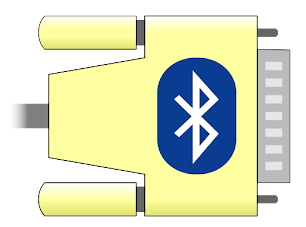
\includegraphics[width=.03\linewidth]{./my-chapters/my-images/implementation/Ble/unnamed.png}) để kiểm tra dữ liệu gửi về smartphone. 

\begin{figure}[H]
	\begin{minipage}{.5\linewidth}
		\centering
		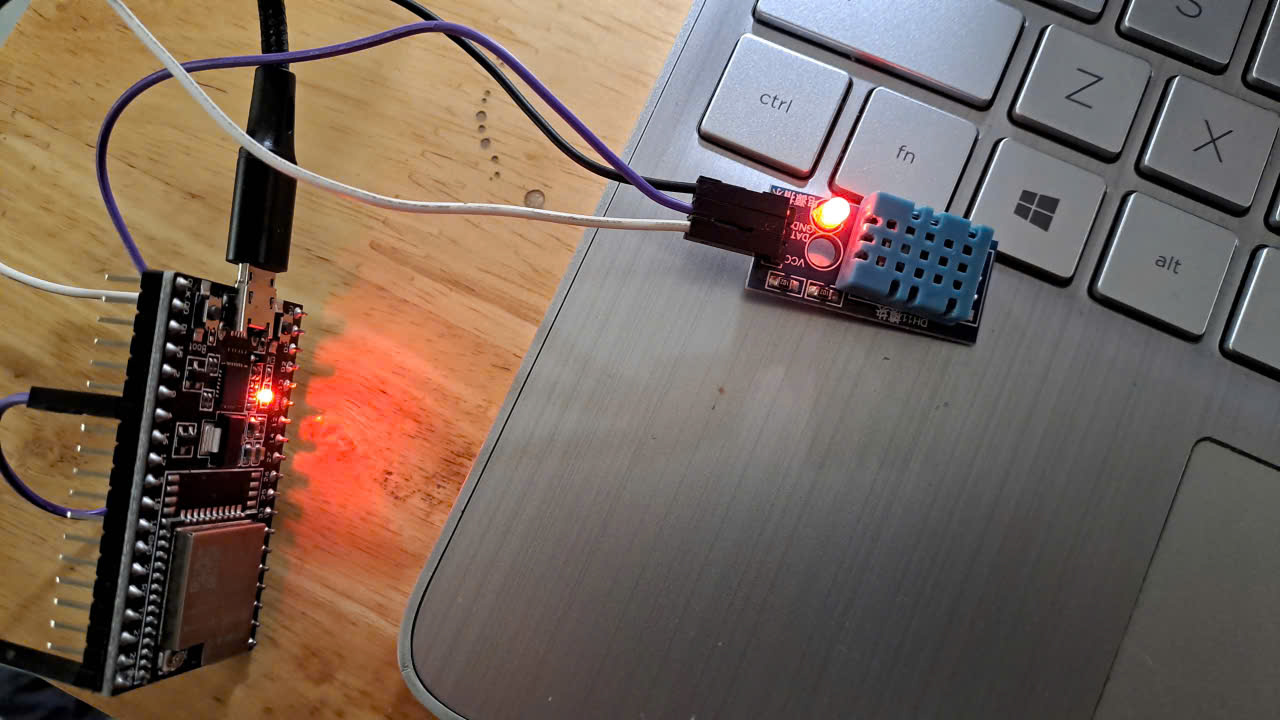
\includegraphics[width=\linewidth]{./my-chapters/my-images/implementation/Ble/anhthucte.jpg}
	\end{minipage}
	\begin{minipage}{.5\linewidth}
		\centering
		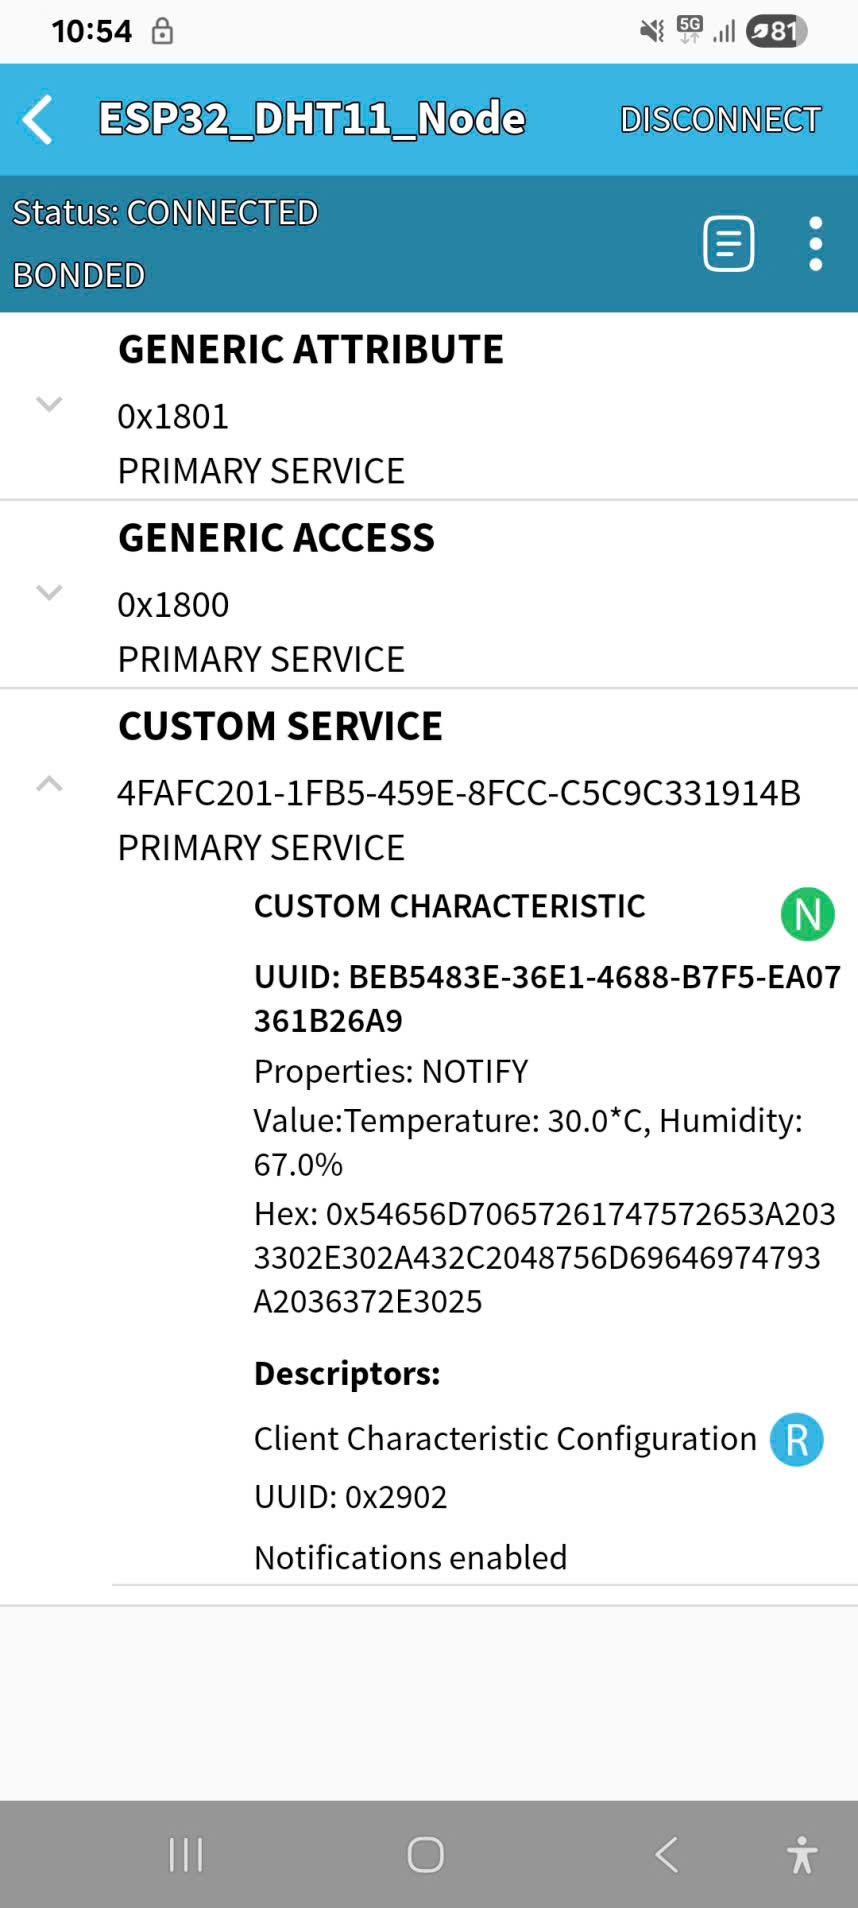
\includegraphics[width=.7\linewidth]{./my-chapters/my-images/implementation/Ble/ketquantrendienthoai.jpg}
	\end{minipage}
	\caption{Hình ảnh thực tế và kết quả kiểm tra đoạn code trên DEVKIT.}
\end{figure}
%\noindent\textbf{Ngắt đánh thức từ bộ WuRx (Wake-up Interrupt GPIO3)}
%
%Trong hệ thống, mạch \textbf{WuRx (Wake-up Receiver)} hoạt động ở mức tiêu thụ điện cực thấp, có nhiệm vụ giám sát tín hiệu RF đầu vào và chỉ đánh thức vi điều khiển khi có dữ liệu hợp lệ. 
%Trên ESP32-C3, chân \textbf{GPIO3} được cấu hình làm ngắt đánh thức ngoài (\textit{External Wake-up EXT0}).
%
%\begin{lstlisting}[language=C, caption={Cấu hình chân GPIO3 làm ngắt đánh thức hệ thống}]
%	#define WURX_PIN 3      // External wake-up interrupt from WuRx
%	esp_sleep_enable_ext0_wakeup((gpio_num_t)WURX_PIN, 0);
%\end{lstlisting}
%
%Khi mạch WuRx phát hiện tín hiệu hợp lệ, nó sẽ kéo mức điện áp trên chân GPIO3 xuống thấp (LOW), từ đó đánh thức MCU thoát khỏi chế độ \textit{Deep Sleep}.
%
%\begin{lstlisting}[language=C, caption={Kiểm tra nguyên nhân đánh thức hệ thống}]
%	esp_sleep_wakeup_cause_t wakeup_reason = esp_sleep_get_wakeup_cause();
%	if (wakeup_reason == ESP_SLEEP_WAKEUP_EXT0)
%	Serial.println("[SYSTEM] Wake-up triggered by WuRx (GPIO3)");
%\end{lstlisting}
%
%Cấu hình này giúp hệ thống hoạt động theo cơ chế \textbf{event-driven}, 
%chỉ tiêu thụ năng lượng khi có sự kiện từ WuRx, 
%từ đó tối ưu hoá \textbf{duty cycle} và kéo dài thời gian hoạt động của cảm biến.
%

\subsubsection{Sơ đồ mạch của một Sensor Node BLE sử dụng chip ESP32-C3}

\begin{figure}[H]
	\centering
	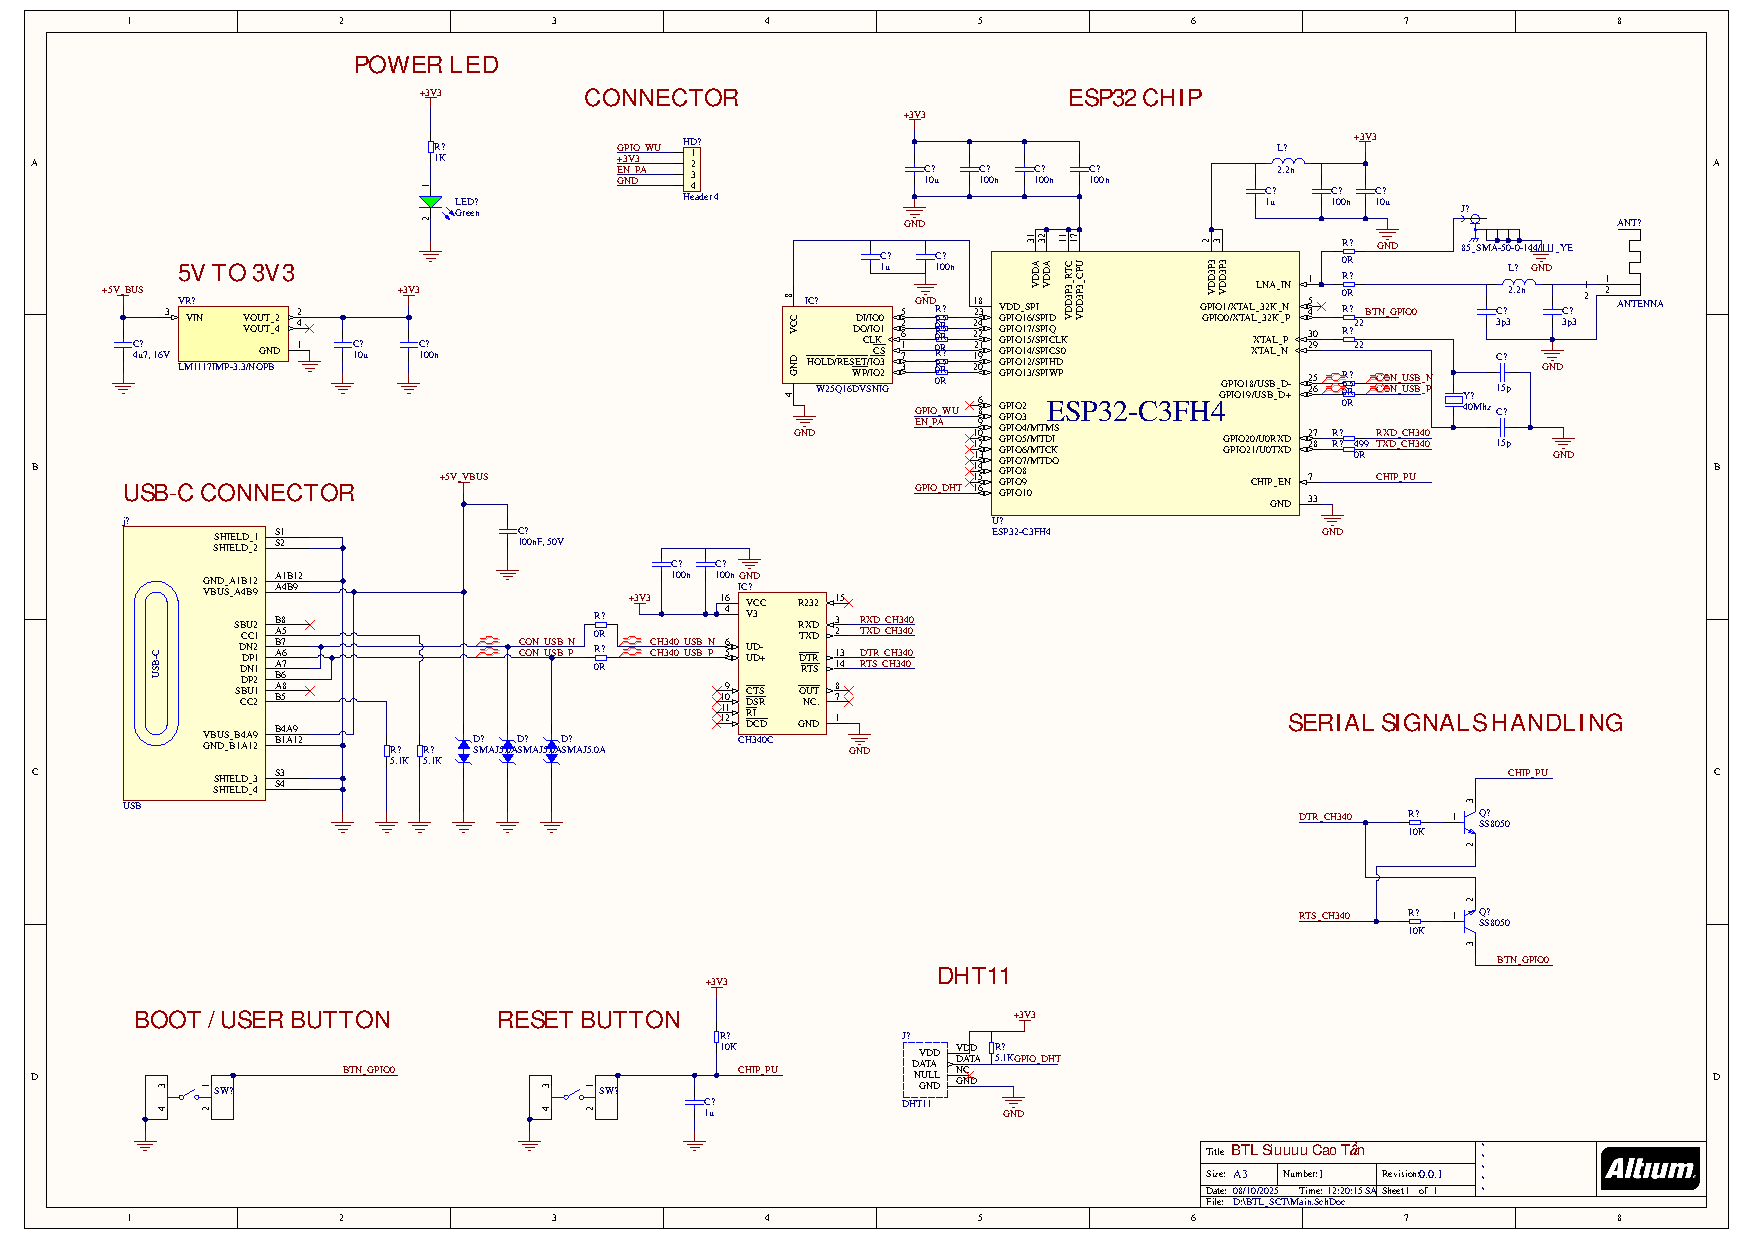
\includegraphics[width=\linewidth]{./my-chapters/my-diagrams/Schematic_for_ESP.pdf}
	\caption{Schematic of a BLE node using ESP32-C3.}
\end{figure}

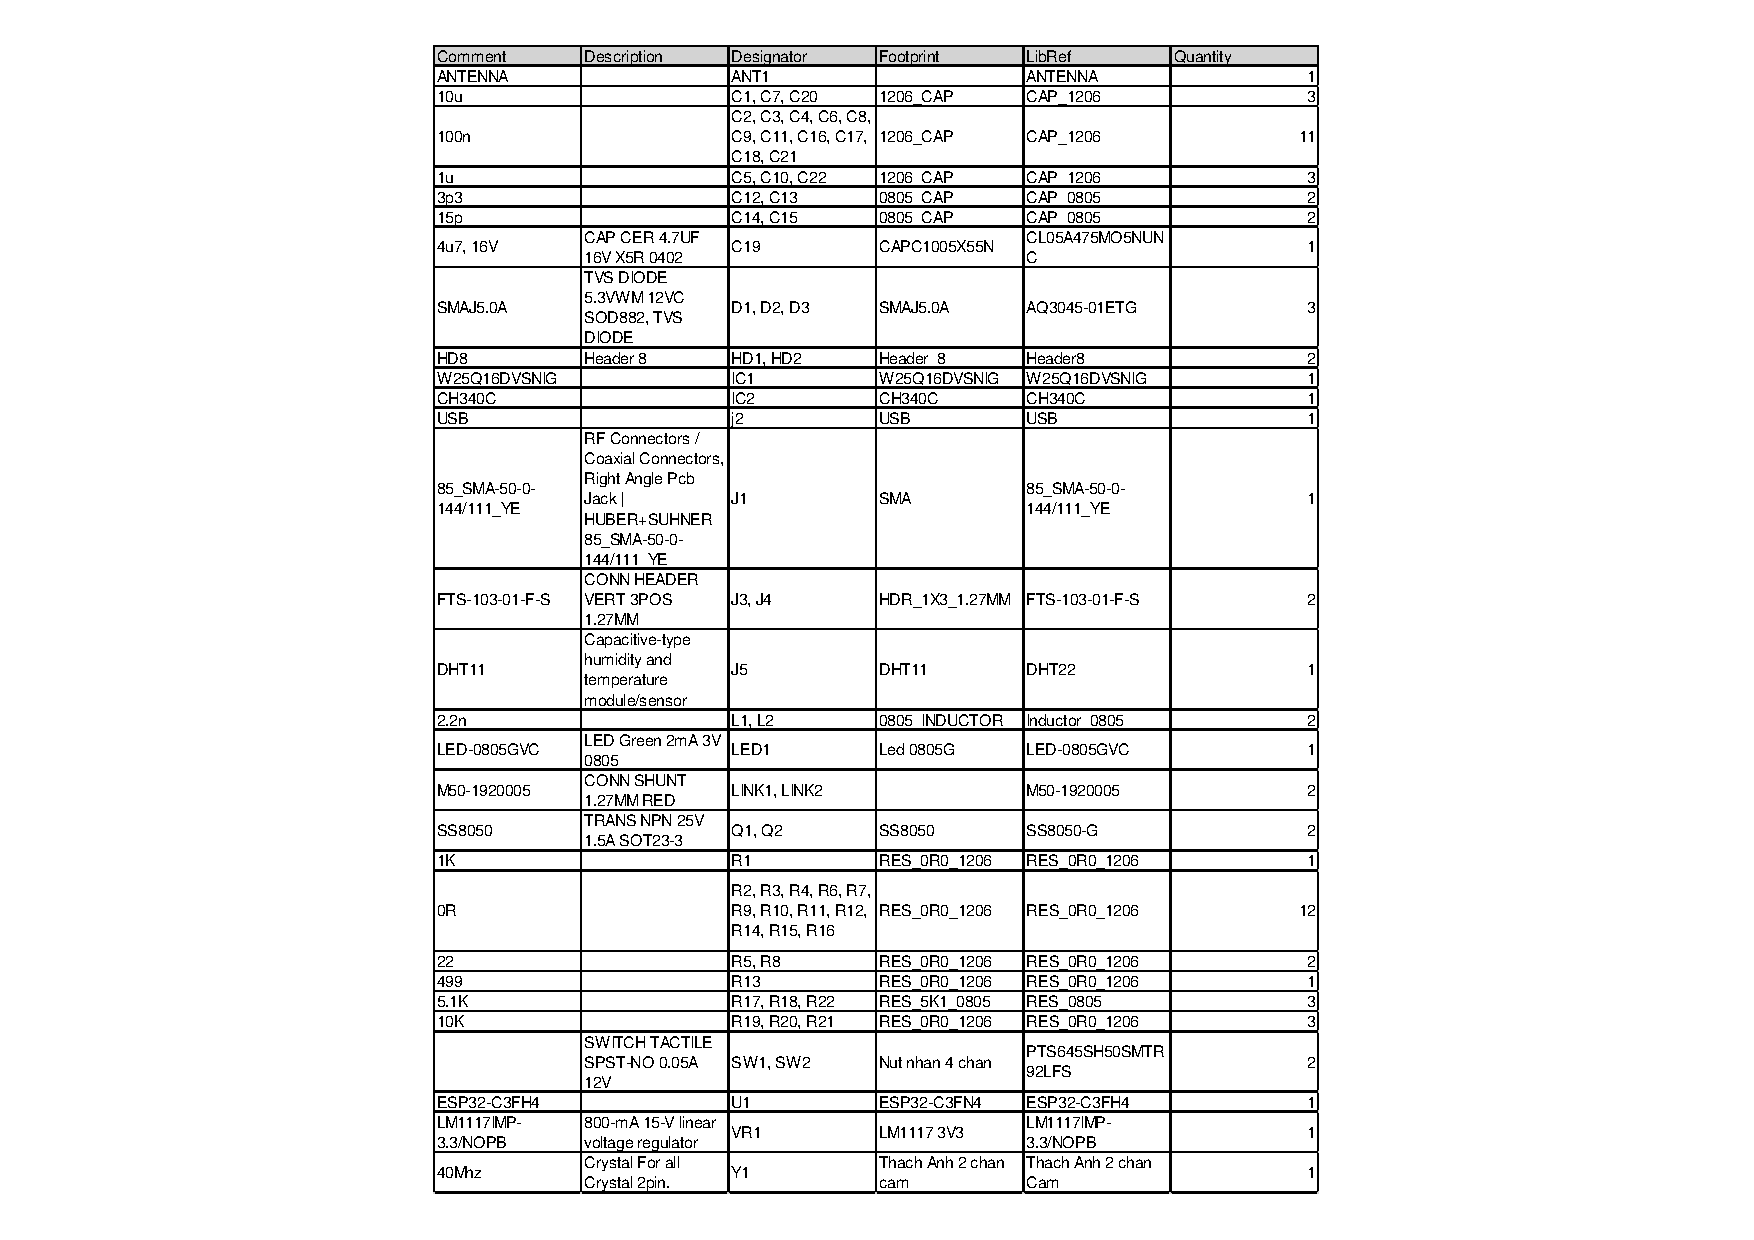
\includegraphics[width=\linewidth]{./my-chapters/my-diagrams/Schematic_for_ESP_1.pdf}

\subsection{Thiết kế Directional Coupler}
\subsubsection{Thiết kế Schematic}

Sử dụng phần mềm Advanced Design System của Keysight để thiết kế Schematic sơ bộ cho Coupled Line Directional Coupler.

\begin{figure}[H]
	\centering
	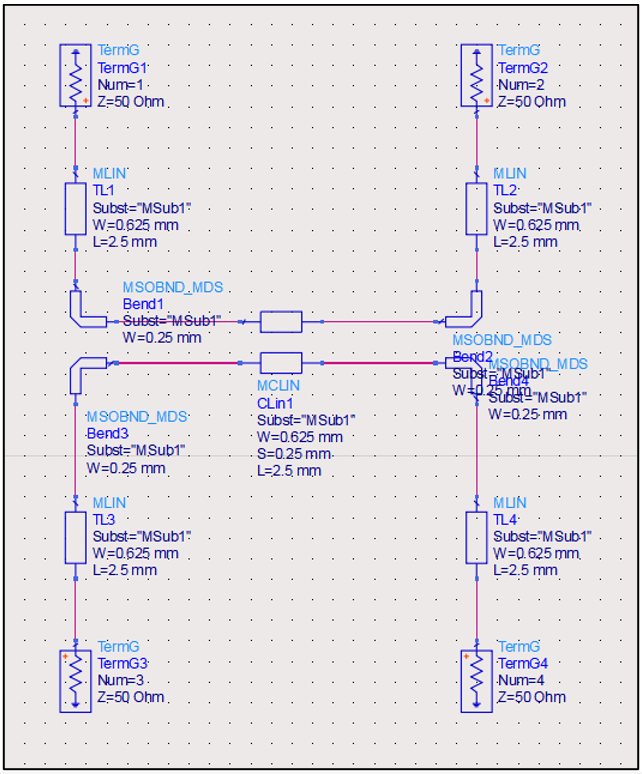
\includegraphics[width=.8\linewidth]{./my-chapters/my-images/implementation/coupler/overview_schemateic_coupler.png}
	\caption{Schematic sơ bộ của Coupled Line Directional Coupler.}
\end{figure}

Sử dụng công cụ LineCalc để tiến hành tính toán các thông số cho Microstrip:

\begin{figure}[H]
	\centering
	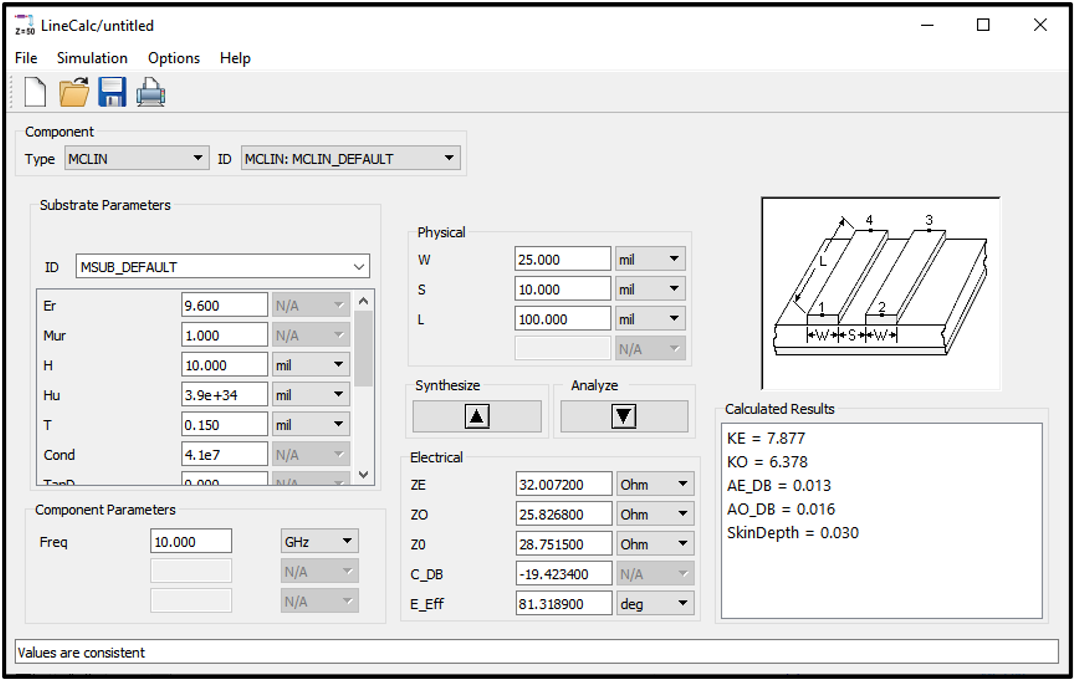
\includegraphics[width=.8\linewidth]{./my-chapters/my-images/implementation/coupler/giaodien.png}
	\caption{Giao diện của LineCalc.}
\end{figure}

Đầu tiên, ta sẽ tính toán thông số cho đường dây trước, để làm được thì ta sẽ xem quy chuẩn PCB của nhà sản xuất PCB trước. Ở đây nhóm chọn Thiên Lam PCB để làm mạch in PCB:

\begin{figure}[H]
	\centering
	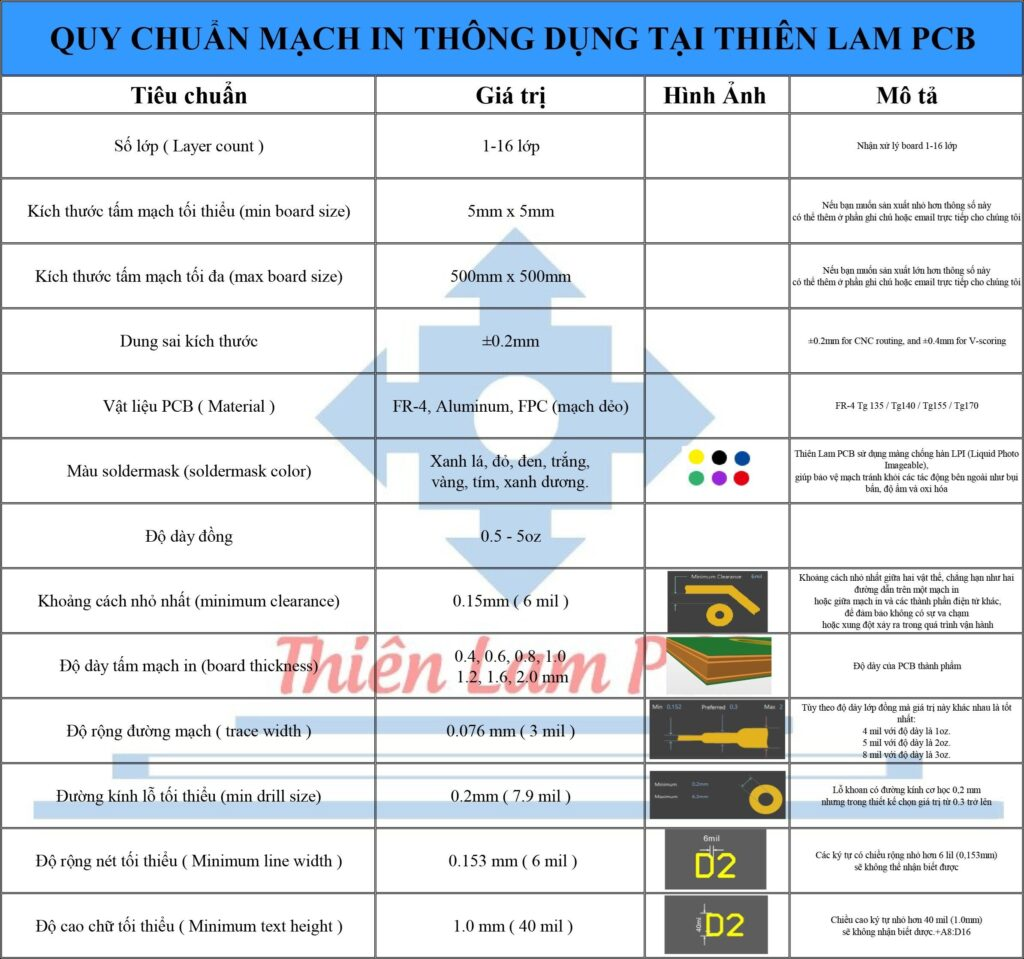
\includegraphics[width=.8\linewidth]{./my-chapters/my-images/implementation/coupler/quychuant_pcd.png}
	\caption{Quy chuẩn mạch in của Thiên Lam PCB.}
\end{figure}

Có thể thấy Thiên Lam PCB sử dụng vật liệu PCB là FR-4 Tg135/140/155/170 với các số thể hiện nhiệt độ mà PCB chịu đựng được. Nhóm sử dụng phíp đồng FR4 độ dày 1.5mm để thực hiện PCB cho Coupler:

\begin{figure}[H]
	\centering
	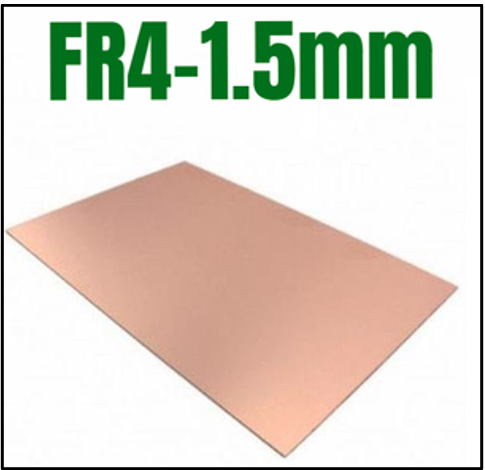
\includegraphics[width=.4\linewidth]{./my-chapters/my-images/implementation/coupler/phipdong_fp4.png}
	\caption{Phíp đồng FR4.}
\end{figure}

\begin{figure}[H]
	\centering
	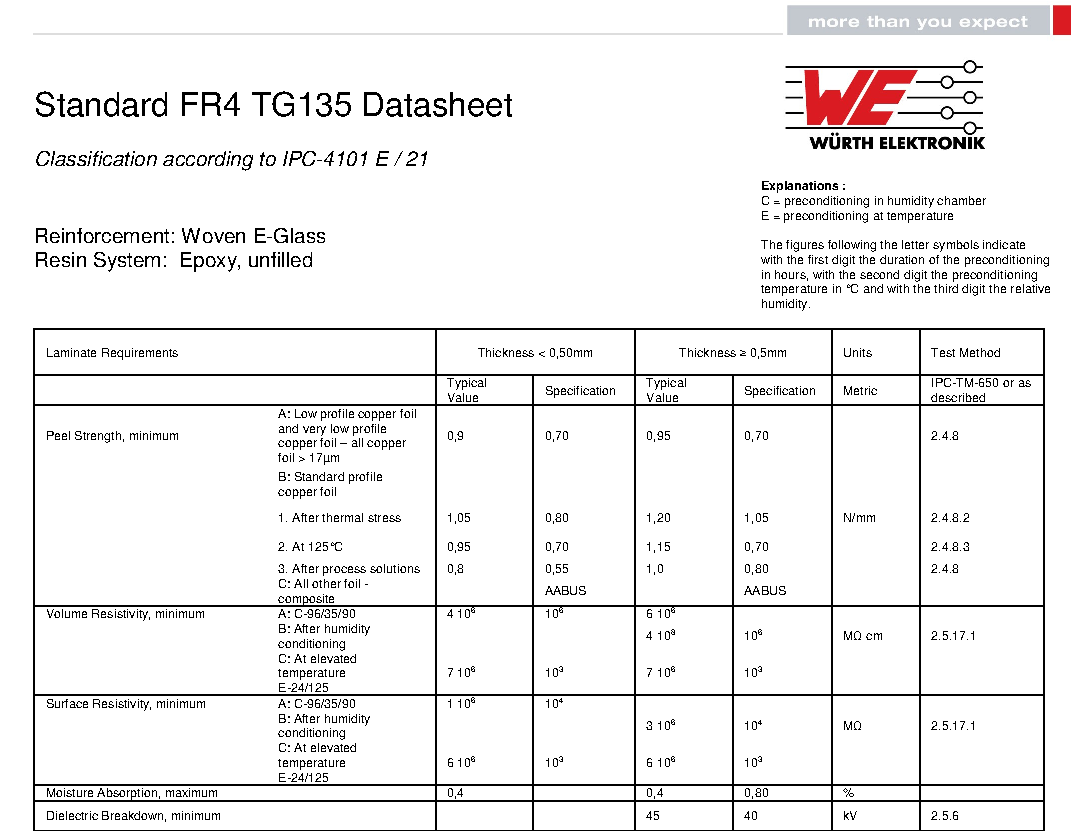
\includegraphics[width=.8\linewidth]{./my-chapters/my-refs/530837204-FR4-Datasheet.pdf}
	\caption{Datasheet của FR4-Tg135.}
\end{figure}

Trong datasheet này, ta chú ý 2 thông số: 

\begin{figure}[H]
	\centering
	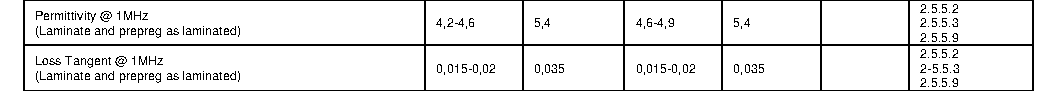
\includegraphics[width=.8\linewidth]{./my-chapters/my-refs/530837204-FR4-Datasheet _Copy.pdf}
	\caption{Thông số độ điện thẩm và hằng số tổn hao.}
\end{figure}

Từ datasheet, với độ dày của board PCB là $1.5\,\textsf{mm}$ nên nhóm sẽ chọn giá trị $Er=4.8$ và $TanD=0.02$.

Sau đó, sử dụng công cụ LineCalc của ADS để thực hiện tính toán kích thước của đường dây microstrip cho Coupler:

\begin{figure}[H]
	\centering
	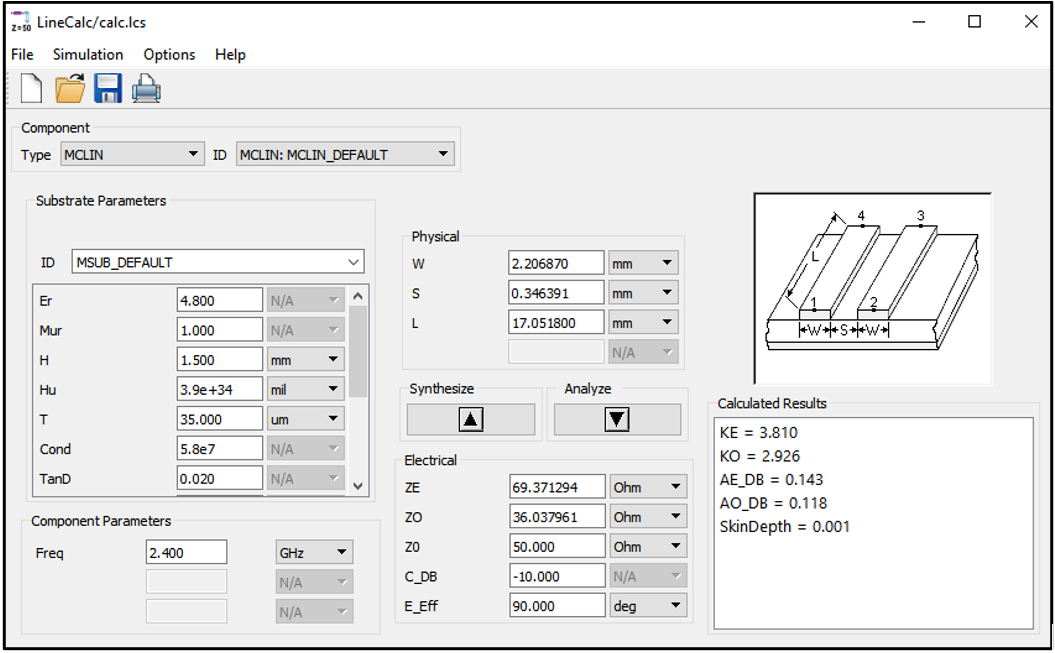
\includegraphics[width=.8\linewidth]{./my-chapters/my-images/implementation/coupler/thogsoduongday.png}
	\caption{Các thông số kích thước đường dây sau khi chạy công cụ LineCalc.}
\end{figure}

Thông số của đường dây:
\begin{itemize}[label=-]
	\item Độ điện thẩm: $\text{Er}=4.8$
	\item Độ dày của bo mạch PCB: $\text{H}=0.6\,\textsf{mm}$
	\item Độ dày của đường microtrip: $\text{T}=35\mu m$
	\item Độ dẫn điện của mircotrip: $\text{Coud} = 5.8 \times 10^{7} \,\textsf{S/m}$ (Đối với microtrip là đồng)
	\item Hệ số tổn hao: $\text{TanD} = 0.02$
	\item Điện trở của đường dây: $Z_{0} = 50\Omega$
	\item Hệ số Coupling: $C=-10dB$ (để lấy ra $1/10$ công suất ngõ vào làm tín hiệu)
\end{itemize}

Từ đó, ta có kích thước của đường dây microstrip coupling:

\begin{itemize}[label=-]
	\item Chiều rộng đường dây: $\text{W} = 2.20687 \,\textsf{mm}$
	\item Chiều dài của cặp dây coupling: $\text{L} = 17.0518\,\textsf{mm}$
	\item Khoảng cách giữa 2 đường dây coupling: $\text{S} = 0.346391\,\textsf{mm}$
\end{itemize}

Thông số đường dây MLIN:

\begin{itemize}[label=-]
	\item Chiều rộng đường dây: $\text{W} = 2.20687 \,\textsf{mm}$
	\item Chiều dài của đường dây: $\text{L} = 7\,\textsf{mm}$
\end{itemize}

\begin{figure}[H]
	\centering
	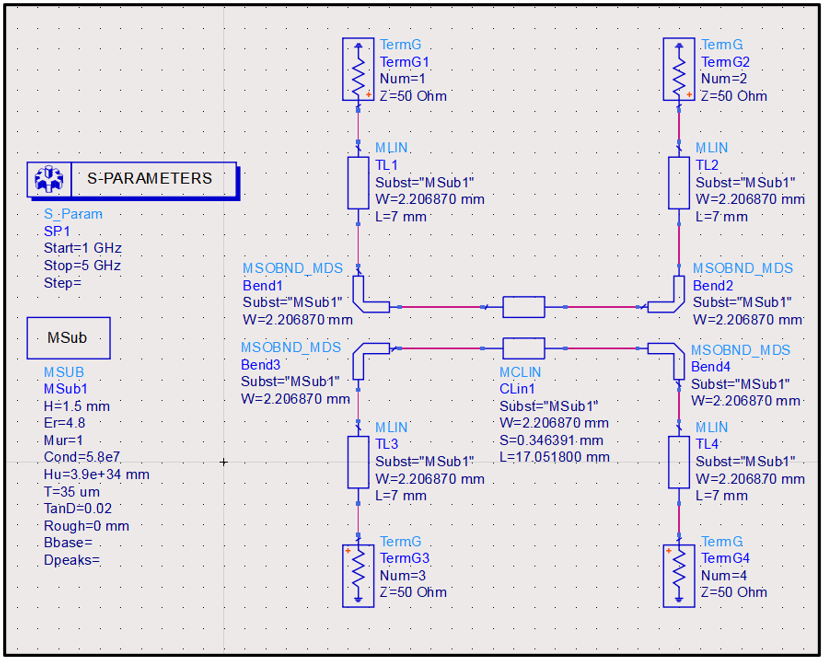
\includegraphics[width=.8\linewidth]{./my-chapters/my-images/implementation/coupler/schematic_saukhi.png}
	\caption{Schematic sau khi đã nhập thông số kích thước của microstrip.}
\end{figure}

Sau đó, tiến hành chạy mô phỏng và kiểm tra kết quả:

\begin{figure}[H]
	\centering
	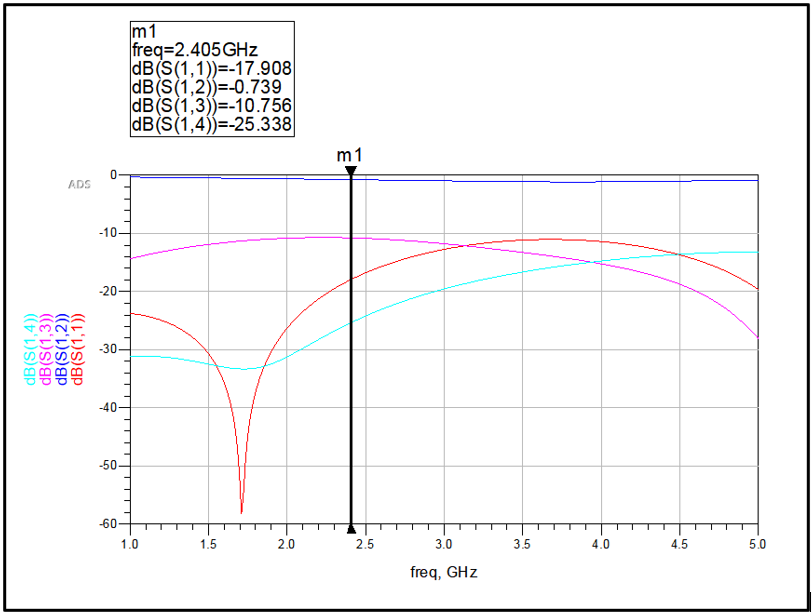
\includegraphics[width=.8\linewidth]{./my-chapters/my-images/implementation/coupler/ketquamophong.png}
	\caption{Kết quả mô phỏng.}
\end{figure}

\textbf{Đánh giá kết quả mô phỏng:}

\begin{table}[H]
	\centering
	\begin{tabular}{|>{\centering\arraybackslash}m{2.5cm}
			|>{\raggedright\arraybackslash}m{3.5cm}
			|>{\centering\arraybackslash}m{3cm}
			|>{\centering\arraybackslash}m{3cm}|}
		\hline
		\textbf{Thông số} 	& \textbf{Kì vọng} 				& \textbf{Đạt được} 		& \textbf{Đánh giá} \\ \hline
		$S_{11}$ 			& Nhỏ hơn $-20 \,\textsf{dB}$	& $-15.806 dB\,\textsf{dB}$ 	& Chưa đạt \\ \hline
		$S_{12}$ 			& Lớn hơn $-1 \,\textsf{dB}$ 	& $-0.584\,\textsf{dB}$	& Đạt \\ \hline
		$S_{13}$ 			& Gần bằng $-10 \,\textsf{dB}$ 	& $-10.649 \,\textsf{dB}$	& Đạt \\ \hline
		$S_{14}$ 			& Nhỏ hơn $-20 \,\textsf{dB}$	& $-23.589 \,\textsf{dB}$	& Đạt \\ \hline
	\end{tabular}
	\caption{Bảng so sánh thông số đo được và kì vọng khi mô phỏng Coupled line Directional Coupler.}
	\label{tab:s_parameters}
\end{table}


\subsubsection{Thiết kế Layout}

Từ những thông số, kích thước đã tính toán ở trên, ta tiến hành vẽ layout trên ADS:

\begin{figure}[H]
	\centering
	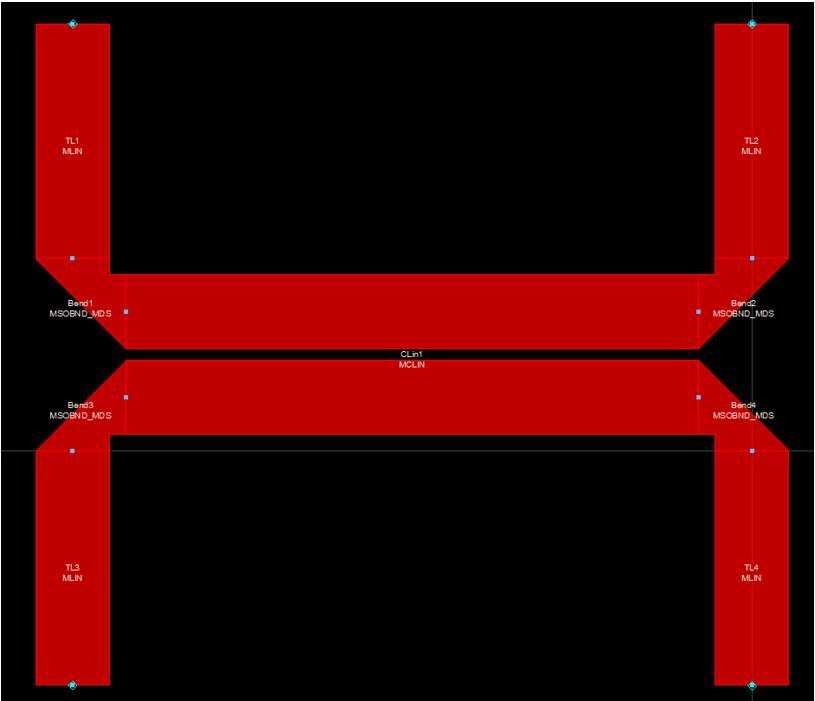
\includegraphics[width=.8\linewidth]{./my-chapters/my-images/implementation/coupler/layout_coupler.png}
	\caption{Layout của Coupled Line Directional Coupler.}
\end{figure}

Sau khi hoàn thành layout, tiến hành chạy mô phỏng và kiểm tra kết quả đạt được:

\begin{figure}[H]
	\centering
	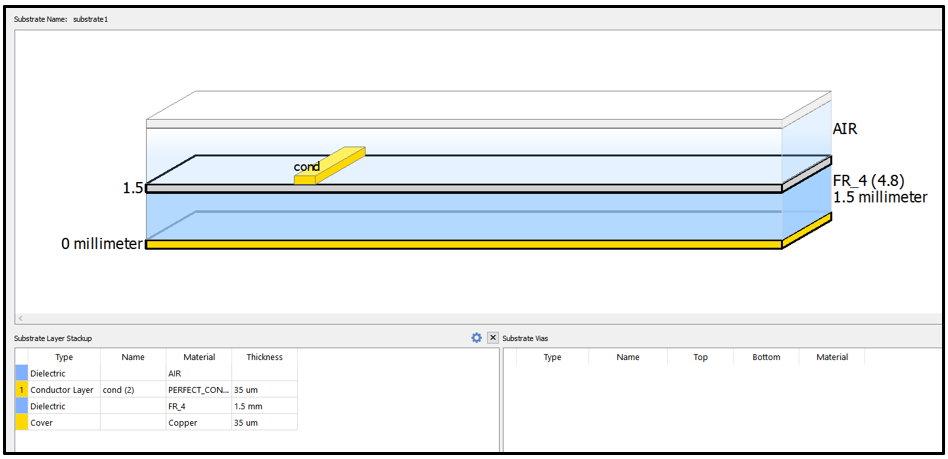
\includegraphics[width=.9\linewidth]{./my-chapters/my-images/implementation/coupler/substrate_pcb.png}
	\caption{Thông số mô phỏng cho substrate của PCB.}
\end{figure}

\begin{figure}[H]
	\centering
	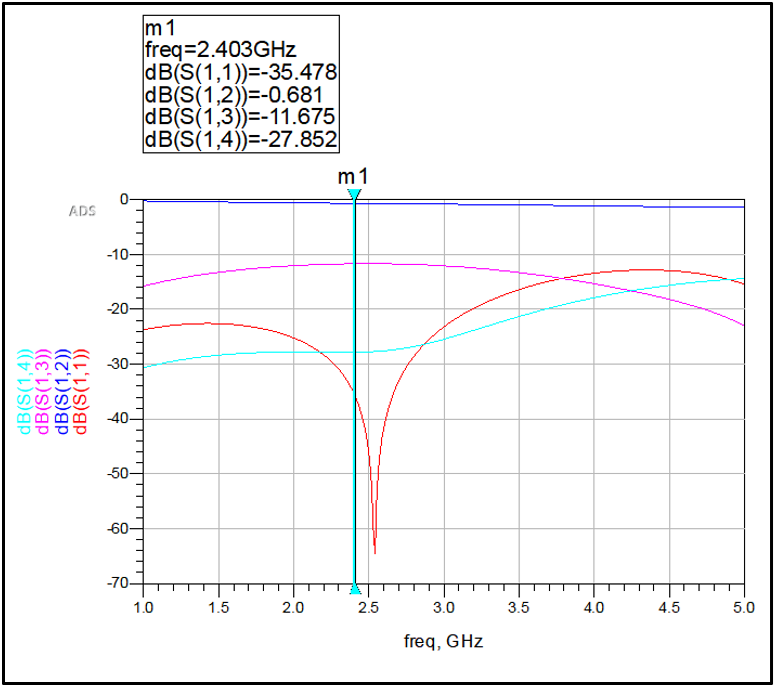
\includegraphics[width=.8\linewidth]{./my-chapters/my-images/implementation/coupler/ketquamophong_layout.png}
	\caption{Kết quả sau khi chạy mô phỏng layout của Coupled Line Directional Coupler.}
\end{figure}

\textbf{Đánh giá kết quả mô phỏng:}

\begin{table}[H]
	\centering
	\begin{tabular}{|>{\centering\arraybackslash}m{2.5cm}
			|>{\raggedright\arraybackslash}m{3.5cm}
			|>{\centering\arraybackslash}m{3cm}
			|>{\centering\arraybackslash}m{3cm}|}
		\hline
		\textbf{Thông số} 	& \textbf{Kì vọng} 				& \textbf{Đạt được} 		& \textbf{Đánh giá} \\ \hline
		$S_{11}$ 			& Nhỏ hơn $-20 \,\textsf{dB}$	& $-35.478 \,\textsf{dB}$ 	& Đạt \\ \hline
		$S_{12}$ 			& Lớn hơn $-1 \,\textsf{dB}$ 	& $-0.681 \,\textsf{dB}$	& Đạt \\ \hline
		$S_{13}$ 			& Gần bằng $-10 \,\textsf{dB}$ 	& $-11.675 \,\textsf{dB}$	& Gần đạt \\ \hline
		$S_{14}$ 			& Nhỏ hơn $-20 \,\textsf{dB}$	& $-27.852 \,\textsf{dB}$	& Đạt \\ \hline
	\end{tabular}
		\caption{Bảng so sánh thông số đo được và kì vọng sau khi chạy mô phỏng layout của Coupled Line Directional Coupler.}
	\label{tab:s_parameters_result}
\end{table}

Qua 2 kết quả mô phỏng trên, ta thấy đư	ợc các thông số khi sử dụng LineCalc chưa được tối ưu, khi vẫn còn các thông số chưa đạt kì vọng. Do đó, ta sử dụng 1 công cụ khác của ADS để đạt được các thông số kì vọng mà ta đặt ra, đó là công cụ Optimization:

\begin{figure}[H]
	\centering
	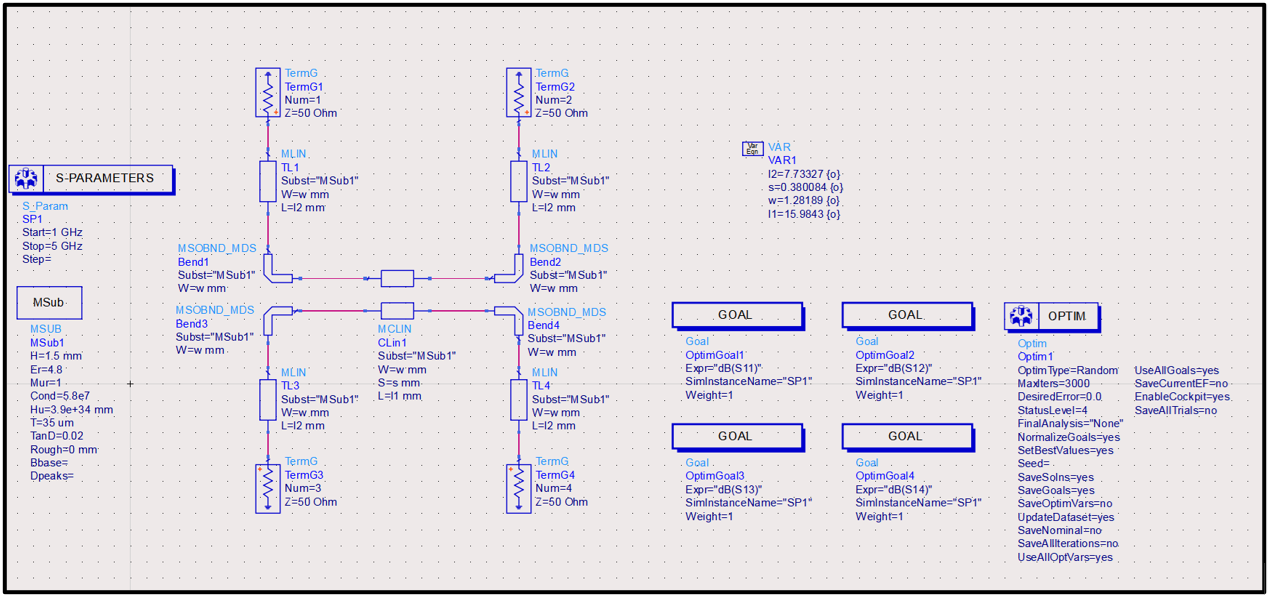
\includegraphics[width=.9\linewidth]{./my-chapters/my-images/implementation/coupler/schematic_optimizetion.png}
	\caption{Schematic với các công cụ Optimization.}
\end{figure}

Đầu tiên, ta sử dụng khối VAR để tạo ra các biến mà ADS được phép thay đổi trong quá trình quá trình tối ưu. Các biến này được khai báo bao gồm giá trị khởi tạo và giới hạn trên/dưới, và sẽ đặt giá trị ban đầu theo thông số tính toán của LineCalc:

\begin{figure}[H]
	\centering
	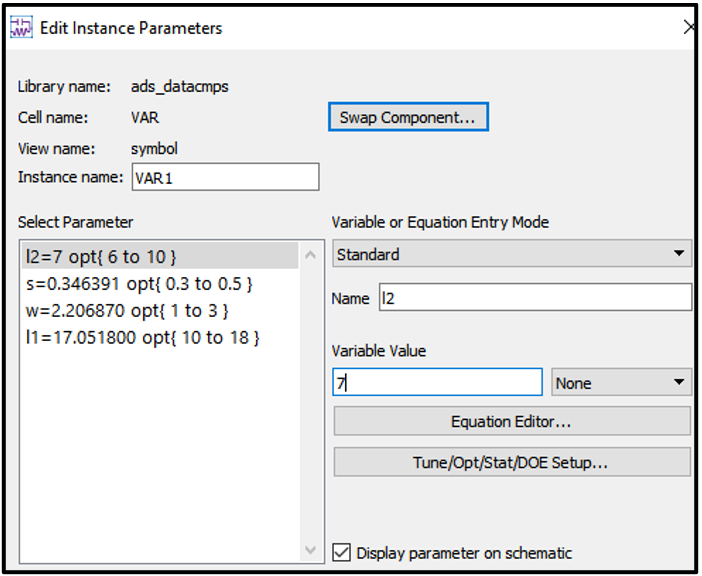
\includegraphics[width=.7\linewidth]{./my-chapters/my-images/implementation/coupler/khoi_VAR.png}
	\caption{Khối VAR tạo các biến.}
\end{figure}

Tiếp theo là khối GOAL để đặt các mục tiêu mà mạch cần đạt được sau khi tối ưu. Ta sẽ đặt các thông số kì vọng như các kết quả mô phỏng ở trên:

\begin{figure}[H]
	\centering
	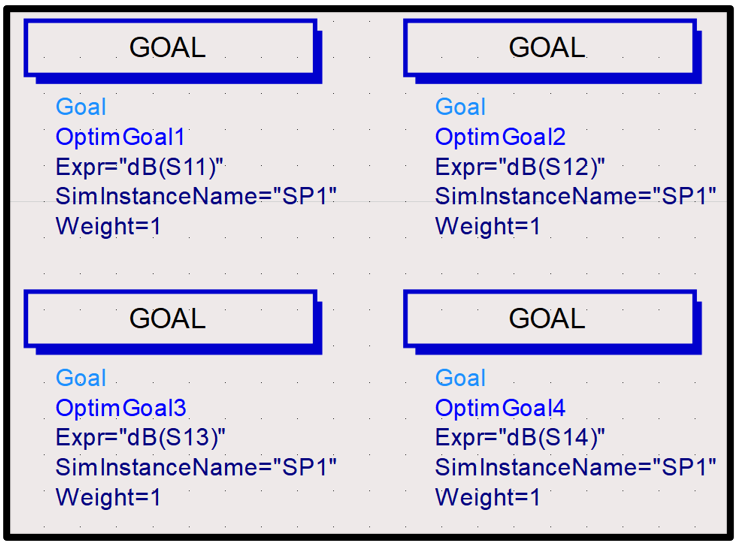
\includegraphics[width=.7\linewidth]{./my-chapters/my-images/implementation/coupler/khoi_global.png}
	\caption{Khối GOAL đặt mục tiêu cần đạt được sau tối ưu.}
\end{figure}

Sau khi thiết lập biến và mục tiêu, khối OPTIM được thêm vào để lựa chọn thuật toán tối ưu phù hợp. Trong sơ đồ mô phỏng bên dưới, khối OPTIM được cấu hình để thực hiện quá trình tối ưu hóa bằng thuật toán Random Optimization. Tham số $MaxIters = 3000$ cho phép bộ tối ưu thực hiện tối đa $3000$ vòng lặp nhằm tìm ra bộ giá trị tốt nhất cho các biến tối ưu.

\begin{figure}[H]
	\centering
	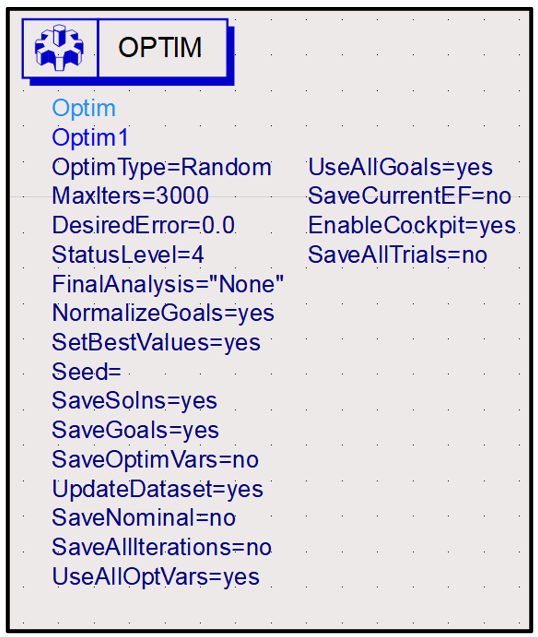
\includegraphics[width=.7\linewidth]{./my-chapters/my-images/implementation/coupler/khoi_OPTIM.png}
	\caption{Khối OPTIM để thực hiện quá trình tối ưu.}
\end{figure}

Sau khi thiết lập xong các công cụ Optimization, ta tiến hành thực hiện tối ưu hoá, tìm ra các thông số tính toán tối ưu nhất để đạt mục tiêu kì vọng:

\begin{figure}[H]
	\centering
	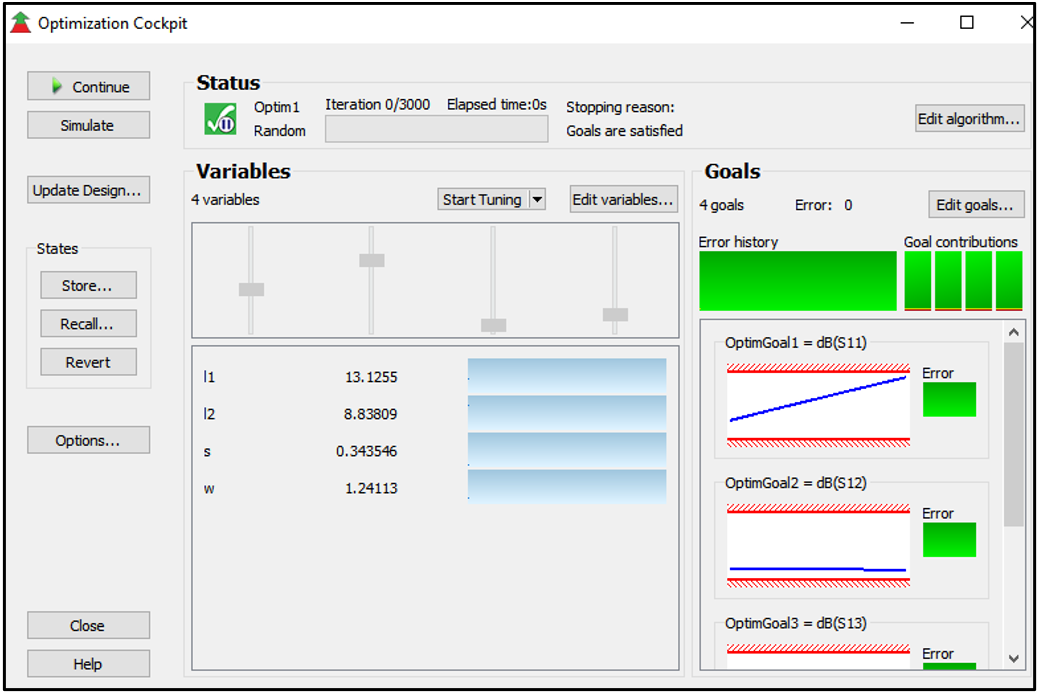
\includegraphics[width=.9\linewidth]{./my-chapters/my-images/implementation/coupler/after_optimazition.png}
	\caption{Kết quả sau khi tối ưu hóa.}
\end{figure}

Tiếp theo, ta tiến hành Update Design để cập nhật các thông số kích thước mới vào Schematic:

\begin{itemize}[label=-]
	\item $W = 1.24113\,\textsf{mm}$
	\item $S = 0.343546\,\textsf{mm}$
	\item $L_{1} = 13.1255\,\textsf{mm}$
	\item $L_{2} =  8.83809\,\textsf{mm}$
\end{itemize}

Kết quả mô phỏng Schematic sau khi tối ưu hoá:

\begin{figure}[H]
	\centering
	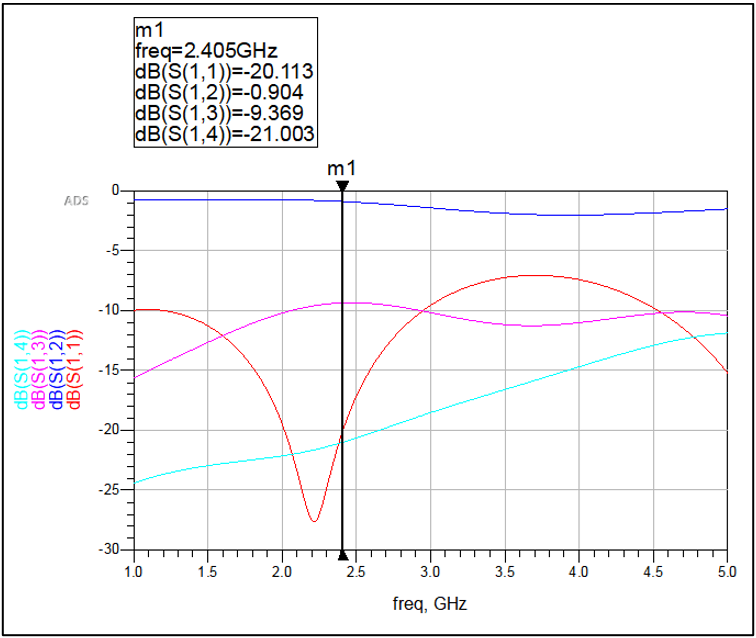
\includegraphics[width=.9\linewidth]{./my-chapters/my-images/implementation/coupler/ketqua_schemati_optimizetion.png}
	\caption{Kết quả mô phỏng Schematic sau khi tối ưu hóa.}
\end{figure}

\textbf{Đánh giá kết quả:}

\begin{table}[H]
	\centering
	\begin{tabular}{|>{\centering\arraybackslash}m{2.5cm}
			|>{\raggedright\arraybackslash}m{3.5cm}
			|>{\centering\arraybackslash}m{3cm}
			|>{\centering\arraybackslash}m{3cm}|}
		\hline
		\textbf{Thông số} 	& \textbf{Kì vọng} 				& \textbf{Đạt được} 		& \textbf{Đánh giá} \\ \hline
		$S_{11}$ 			& Nhỏ hơn $-20 \,\textsf{dB}$	& $-20.113 \,\textsf{dB}$ 	& Đạt \\ \hline
		$S_{12}$ 			& Lớn hơn $-1 \,\textsf{dB}$ 	& $-0.904 \,\textsf{dB}$	& Đạt \\ \hline
		$S_{13}$ 			& Gần bằng $-10 \,\textsf{dB}$ 	& $-9.369 \,\textsf{dB}$	& Chấp nhận được\\ \hline
		$S_{14}$ 			& Nhỏ hơn $-20 \,\textsf{dB}$	& $-21.003 \,\textsf{dB}$	& Đạt \\ \hline
	\end{tabular}
	\caption{Bảng so sánh thông số đo được và kì vọng khi mô phỏng Coupled line Directional Coupler sau khi Optimization.}
\end{table}

\begin{figure}[H]
	\centering
	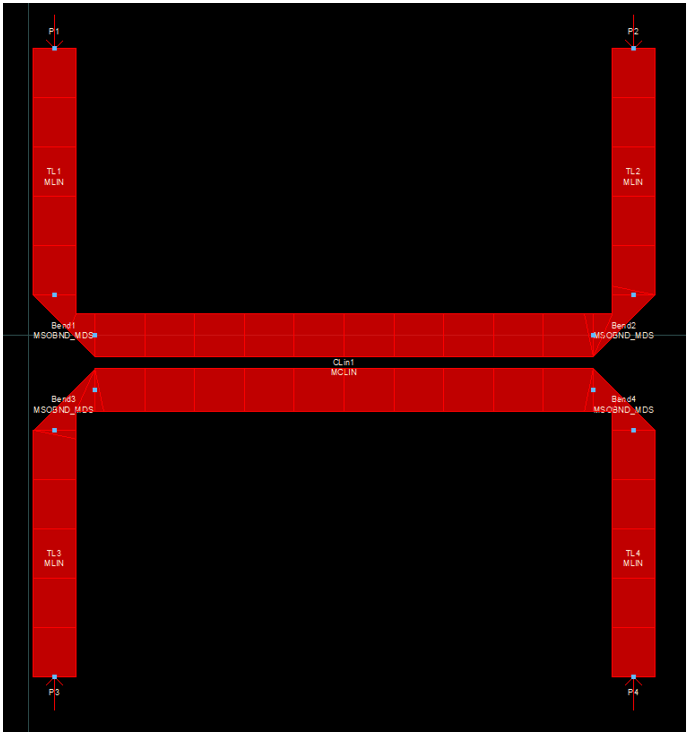
\includegraphics[width=.9\linewidth]{./my-chapters/my-images/implementation/coupler/layout_coupler_optimazition.png}
	\caption{Layout với các thông số kích thước tối ưu hoá.}
\end{figure}

\begin{figure}[H]
	\centering
	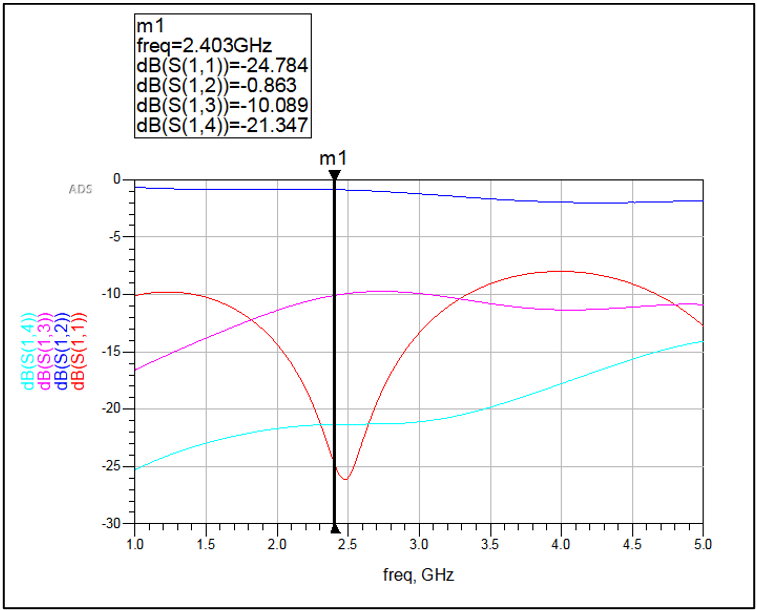
\includegraphics[width=.9\linewidth]{./my-chapters/my-images/implementation/coupler/ketqua_layout_optimizetion.png}
	\caption{Kết quả mô phỏng Layout sau khi tối ưu hoá.}
\end{figure}

\begin{table}[H]
	\centering
	\begin{tabular}{|>{\centering\arraybackslash}m{2.5cm}
			|>{\raggedright\arraybackslash}m{3.5cm}
			|>{\centering\arraybackslash}m{3cm}
			|>{\centering\arraybackslash}m{3cm}|}
		\hline
		\textbf{Thông số} 	& \textbf{Kì vọng} 				& \textbf{Đạt được} 		& \textbf{Đánh giá} \\ \hline
		$S_{11}$ 			& Nhỏ hơn $-20 \,\textsf{dB}$	& $-24.784 \,\textsf{dB}$ 	& Đạt \\ \hline
		$S_{12}$ 			& Lớn hơn $-1 \,\textsf{dB}$ 	& $-0.863 \,\textsf{dB}$	& Đạt \\ \hline
		$S_{13}$ 			& Gần bằng $-10 \,\textsf{dB}$ 	& $-10.089 \,\textsf{dB}$	& Đạt \\ \hline
		$S_{14}$ 			& Nhỏ hơn $-20 \,\textsf{dB}$	& $-21.347 \,\textsf{dB}$	& Đạt \\ \hline
	\end{tabular}
	\caption{Bảng so sánh thông số đo được và kì vọng sau khi chạy mô phỏng layout của Coupled Line Directional Coupler sau khi Optimization.}
\end{table}